\chapter{Psalm 53}

\begin{figure}
  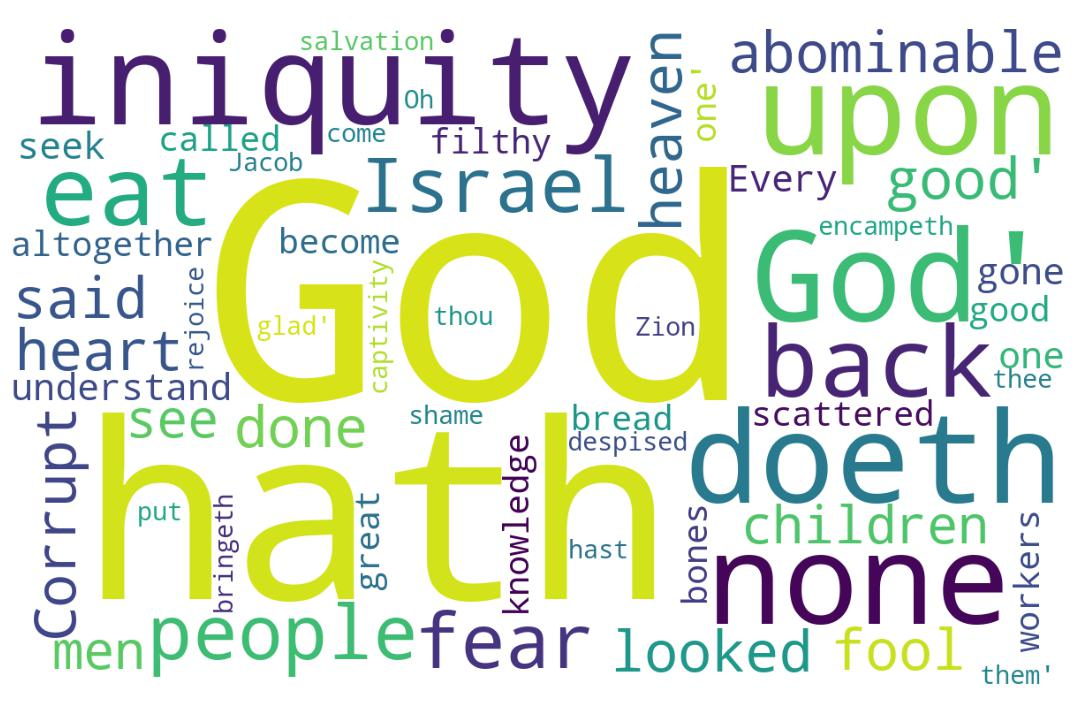
\includegraphics[width=\linewidth]{19OT-Psalms/Psalm53-WordCloud.jpg}
  \caption{Psalm 53 Word Cloud}
  \label{fig:Psalm 53 word Cloud}
\end{figure}


\marginpar{\scriptsize \centering \fcolorbox{bone}{lime}{\textbf{FOOLS AND SAINTS}}\\ (Psalm 53:1-6) \begin{compactenum}[I.][8]
    \item A \textbf{Foolish Saying} \index[scripture]{Psalms!Psa 053:01} (Psa 53:1)
    \item A \textbf{Frustrating Search} \index[scripture]{Psalms!Psa 053:02} (Psa 53:2)
    \item \textbf{Filthy Sinners}  \index[scripture]{Psalms!Psa 053:03} (Psa 53:3)
    \item \textbf{Fearful and Scattered}  \index[scripture]{Psalms!Psa 053:05} (Psa 53:5)
    \item \textbf{Future Society}  \index[scripture]{Psalms!Psa 053:06} (Psa 53:6)
    \item \textbf{Family of Saints}  \index[scripture]{Psalms!Psa 014:05} (Psa 14:5)
\end{compactenum}}


\footnote{\textcolor[cmyk]{0.99998,1,0,0}{\hyperlink{TOC}{Return to end of Table of Contents.}}}\footnote{\href{https://audiobible.com/bible/psalms_53.html}{\textcolor[cmyk]{0.99998,1,0,0}{Psalms  Audio}}}\textcolor[cmyk]{0.99998,1,0,0}{The fool hath said in his heart, \fcolorbox{bone}{lime}{\emph{There} \emph{is} no God}. Corrupt are they, and have done abominable iniquity: \emph{there} \emph{is} none that doeth good.}\footnote{\textbf{Psalm 14:1-7} - The fool hath said in his heart, There is no God. They are corrupt, they have done abominable works, there is none that doeth good. [2] The LORD looked down from heaven upon the children of men, to see if there were any that did understand, and seek God. [3] They are all gone aside, they are all together become filthy: there is none that doeth good, no, not one. [4 Have all the workers of iniquity no knowledge? who eat up my people as they eat bread, and call not upon the LORD. [5] There were they in great fear: for God is in the generation of the righteous. [6] Ye have shamed the counsel of the poor, because the LORD is his refuge. [7] Oh that the salvation of Israel were come out of Zion! when the LORD bringeth back the captivity of his people, Jacob shall rejoice, and Israel shall be glad.}\footnote{\textbf{Proverbs 18:1--3} -- Through desire a man, having separated himself, seeketh and intermeddleth with all wisdom.  [2]  A fool hath no delight in understanding, but that his heart may discover itself. [3] When the wicked cometh, then cometh also contempt, and with ignominy reproach.}
[2] \textcolor[cmyk]{0.99998,1,0,0}{God looked down from heaven upon the children of men, \fcolorbox{bone}{lime}{to see} if there were \emph{any} that did understand, that did seek God.}\footnote{\textbf{Psalm 11:4} - The LORD is in his holy temple, the LORD'S throne is in heaven: his eyes behold, his eyelids try, the children of men.}\footnote{\textbf{Psalm 33:13-14} - The LORD looketh from heaven; he beholdeth all the sons of men. [14] From the place of his habitation he looketh upon all the inhabitants of the earth.}\footnote{\textbf{Psalm 102:19} - For he hath looked down from the height of his sanctuary; from heaven did the LORD behold the earth;}\footnote{\textbf{Jeremiah 16:17} - For mine eyes are upon all their ways: they are not hid from my face, neither is their iniquity hid from mine eyes.}\footnote{\textbf{Jeremiah 23:24} - Can any hide himself in secret places that I shall not see him? saith the LORD. Do not I fill heaven and earth? saith the LORD.}
[3] \textcolor[cmyk]{0.99998,1,0,0}{\fcolorbox{bone}{lime}{Every one} of them is gone back: they are altogether become filthy; \emph{there} \emph{is} none that doeth good, no, not one.}
[4] \textcolor[cmyk]{0.99998,1,0,0}{Have the workers of iniquity no knowledge? who eat up my people \emph{as} they eat bread: they have not called upon God.}\footnote{\textbf{Psalm 94:8} - Understand, ye brutish among the people: and ye fools, when will ye be wise?}\footnote{\textbf{Isaiah 27:11} - When the boughs thereof are withered, they shall be broken off: the women come, and set them on fire: for it is a people of no understanding: therefore he that made them will not have mercy on them, and he that formed them will shew them no favour.}\footnote{\textbf{Jeremiah 4:22} - For my people is foolish, they have not known me; they are sottish children, and they have none understanding: they are wise to do evil, but to do good they have no knowledge.}\footnote{\textbf{Psalm 27:2} - When the wicked, even mine enemies and my foes, came upon me to eat up my flesh, they stumbled and fell.}\footnote{\textbf{Jeremiah 10:25} - Pour out thy fury upon the heathen that know thee not, and upon the families that call not on thy name: for they have eaten up Jacob, and devoured him, and consumed him, and have made his habitation desolate.}\footnote{\textbf{Revelation 17:16} - And the ten horns which thou sawest upon the beast, these shall hate the whore, and shall make her desolate and naked, and shall eat her flesh, and burn her with fire.}
[5] \textcolor[cmyk]{0.99998,1,0,0}{There were they in \fcolorbox{bone}{lime}{great fear}, \emph{where} no fear was: for God hath scattered the bones of him that encampeth \emph{against} thee: thou hast put \emph{them} to shame, because God hath despised them.}
[6] \textcolor[cmyk]{0.99998,1,0,0}{Oh that the \fcolorbox{bone}{lime}{salvation} of Israel \emph{were} \emph{come} out of Zion! When God bringeth back the captivity of his people, Jacob shall rejoice, \emph{and} Israel shall be glad.}\footnote{\textbf{Psalm 14:7} - Oh that the salvation of Israel were come out of Zion! when the LORD bringeth back the captivity of his people, Jacob shall rejoice, and Israel shall be glad.}\footnote{\textbf{Psalm 50:2} - Out of Zion, the perfection of beauty, God hath shined.}\footnote{\textbf{Psalm 85:1} - LORD, thou hast been favourable unto thy land: thou hast brought back the captivity of Jacob.}\footnote{\textbf{Job 42:10} -  And the LORD turned the captivity of Job, when he prayed for his friends: also the LORD gave Job twice as much as he had before.}\footnote{\textbf{Psalm 126:1-4} - When the LORD turned again the captivity of Zion, we were like them that dream. [2] Then was our mouth filled with laughter, and our tongue with singing: then said they among the heathen, The LORD hath done great things for them. [3] The LORD hath done great things for us; whereof we are glad. 4 Turn again our captivity, O LORD, as the streams in the south. }\footnote{\textbf{Jeremiah 30:18} - Thus saith the LORD; Behold, I will bring again the captivity of Jacob's tents, and have mercy on his dwellingplaces; and the city shall be builded upon her own heap, and the palace shall remain after the manner thereof.}\footnote{\textbf{Jeremiah 31:23} - Thus saith the LORD of hosts, the God of Israel; As yet they shall use this speech in the land of Judah and in the cities thereof, when I shall bring again their captivity; The LORD bless thee, O habitation of justice, and mountain of holiness.}\footnote{\textbf{Joel 3:1} - For, behold, in those days, and in that time, when I shall bring again the captivity of Judah and Jerusalem,}\footnote{\textbf{Amos 9:14} - And I will bring again the captivity of my people of Israel, and they shall build the waste cities, and inhabit them; and they shall plant vineyards, and drink the wine thereof; they shall also make gardens, and eat the fruit of them.}



